% REMEMBER: You must not plagiarise anything in your report. Be extremely careful.

\documentclass{l4proj}

    
%
% put any additional packages here
%

\begin{document}

%==============================================================================
%% METADATA
\title{Espruino Tools - An asynchronous JavaScript library to control remote embedded devices [JavaScript, Promise, Arduino]}
\author{Callum McLuskey}
\date{Month 00, 2023}

\maketitle

%==============================================================================
%% ABSTRACT
\begin{abstract}
    \textbf{THIS IS UNFINISHED}

    The personal usage of remote embedded devices is a growing area in engineering allowing for anybody to get started building robotics systems at home or even develop skill sets in programming and electronic engineering. A big name in this scene is Arduino a product which allows hobbyists to build and design systems to suit personal project needs; The Espruino project takes this in a different direction by utilising a javascript interpreter which aims to bring remote embedded systems programming to the web. This project intends to improve the development experience of remote embedded devices by refining the process and allowing users to focus more on their ideas and less on the semantics required to implement them. To achieve this the project introduces many packages providing functionality such as easy device connection[ADD LINK], peer-to-peer[ADD LINK] connection for mobile device inputs to be used, and the refined syntax to allow developers to get started regardless of skill or prior knowledge with wide and detailed documentation to avoid confusion when developing. In addition to this to further ease development, a CLI tool has been developed to create projects preset with all the functionality a beginner user could need, setting anybody up for programming Espruino devices, an activity which had no clear direction before of how to be done. By utilising user studies throughout the project a variety of users from different experience levels have been considered during the development process allowing for the project to be as accessible as possible.

\end{abstract}

\def\consentname {Callum McLuskey} % your full name
\def\consentdate {XX March 2023} % the date you agree

\educationalconsent

\tableofcontents

%==============================================================================
%% Notes on formatting
%==============================================================================
% The first page, abstract and table of contents are numbered using Roman numerals and are not
% included in the page count. 
%
% From now on pages are numbered
% using Arabic numerals. Therefore, immediately after the first call to \chapter we need the call
% \pagenumbering{arabic} and this should be called once only in the document. 
%
% Do not alter the bibliography style.
%
% The first Chapter should then be on page 1. You are allowed 40 pages for a 40 credit project and 30 pages for a 
% 20 credit report. This includes everything numbered in Arabic numerals (excluding front matter) up
% to but excluding the appendices and bibliography.
%
% You must not alter text size (it is currently 10pt) or alter margins or spacing.
%
%
%==================================================================================================================================
%
% IMPORTANT
% The chapter headings here are **suggestions**. You don't have to follow this model if
% it doesn't fit your project. Every project should have an introduction and conclusion,
% however. 
%
%==================================================================================================================================
\chapter{Introduction}

% reset page numbering. Don't remove this!
\pagenumbering{arabic} 


\section{Motivation}

\textbf{[THIS IS A PLACEHOLDER NEEDS EXPANDING]}

\text Remote embedded systems is a sector of engineering which provides developers with a hands on experience allowing for code to be developed into a tangible object providing developers with a rewarding end product.However  the  currently  implementations  of  this  such  as  Arduino  have  a  high  learning  curve  using  C++ as the language to program their devices or micro python which while removing the high learning curve leaves developers with non-transferable skills due to its high abstraction from the core python language.By working with the Espruino catalog of devices we by pass these issues.  Despite this development with Espruino devices still provides a closed in understanding of how JavaScript works leaving the developer with  non  transferable  skills.   This  project  helps  prepare  future  programmers  and  software  engineers  for work within the embedded systems allowing them to achieve working systems as well as allowing for the development of in demand skills through the usage of modern JavaScript with easy access to work with any modern JavaScript of their choice.

\section{Aims / Goals}

\textbf{[THIS IS A PLACEHOLDER NEEDS EXPANDING]}

\text This project will provide an ecosystem of packages to reduce the entry barrier to remote embedded systems programming whilst allowing experienced developers to still benefit from the ease of life additions brought forth with them.  On top of this these packages are built with web technologies at the fore front allowing both experienced and new developers to improve their grasp on current web technologies while developing their embedded systems



%==================================================================================================================================
\chapter{Background}

\textbf{NONE OF THIS IS FINAL AND NEEDS TO BE REWRITTEN}

\section{Espruino Devices}
\text 
The Espruino micro-controller provides an innovative solution for individuals seeking to materialise their electronics project aspirations. With a JavaScript interpreter and in-built amenities such as WiFi and Bluetooth, this device makes it effortless for individuals of diverse programming proficiency to dive in. The Espruino ecosystem caters to both hobbyists and students who are eager to learn about electronics and programming. These micro-controllers can be blended seamlessly with other hardware and software systems, opening up a world of possibilities for electronics projects.
    
\section{UART}
\text UART, or Universal Asynchronous Receiver/Transmitter, is a widely used communication protocol in the world of microcontrollers and embedded systems. It doesn't require a fixed clock rate between the sender and receiver and instead uses start and stop bits for data transmission synchronization.

\begin{figure}
    \centering
    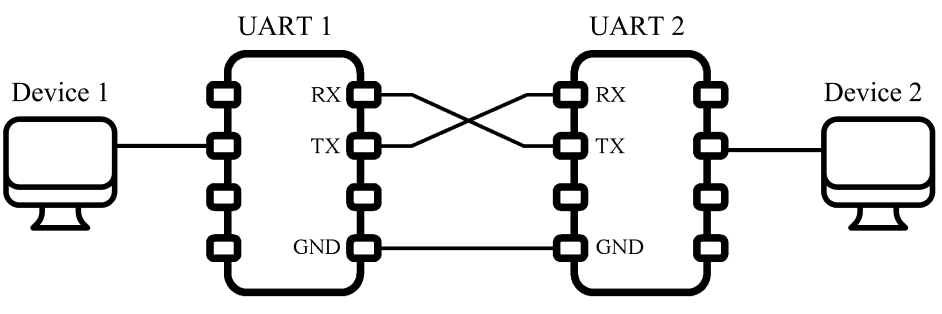
\includegraphics[width=60mm,scale=0.5]{dissertation/images/UART_diagram.png}

    \caption{UART communication}
    \label{fig:my_label}
\end{figure}


\section{WebBluetooth}
\text WebBluetooth is an aspect of the Web API that facilitates communication between web applications and Bluetooth Low Energy (BLE) devices. This technology allows web developers to control and access BLE devices using JavaScript, providing a streamlined and standardized approach.

WebBluetooth represents a milestone in the integration of BLE devices into the web, as it offers a common platform for web developers to interact with these devices, regardless of their origin or operating system. It expands the possibilities for BLE devices, including the ability to control smart home technology or track fitness information through a web application.

\section{NPM}
\text NPM is a tool utilized in the world of JavaScript programming to manage software packages. It serves as a centralized hub for individuals to quickly find, install, and handle an extensive collection of libraries and packages for their projects. NPM empowers developers to share their packages and work together on open-source initiatives. Due to its large repository of packages, NPM has become a must-have tool for contemporary JavaScript development.

\section{NPX}
\text NPX is a tool for executing Node.js packages, including those installed through npm (Node Package Manager). It allows users to run a package's binary without having to install it globally on their system. This is useful for testing packages or trying out new features without affecting other parts of the system. NPX also enables developers to run packages with specific versions, rather than relying on the globally installed version. It provides a convenient and efficient way to run packages, making it a popular tool in the Node.js ecosystem.

\section{WebRTC}
\text WebRTC (Web Real-Time Communication) is a freely available resource that enables web browsers and devices to communicate voice, video and data in real-time without the need for additional software. This technology has been engineered to operate on a variety of networks and platforms, resulting in low lag and excellent audio and video streaming quality for web-based communication. Popular uses for WebRTC include video conferencing, live streaming, online gaming, and file sharing.

\section{Open Source}
\text Open source pertains to a licensing model for software that enables the public to view and modify the source code. It is developed and maintained by a community of contributors, rather than by a single entity. The objective of open source is to promote collaboration, transparency, and innovation in software development, and to give users more control and choice over their software. Notable open source projects include the Linux operating system and the Python programming language.

\section{Existing Projects}
\text Espruino native language / online IDE.

%==================================================================================================================================
\chapter{Analysis/Requirements}
What is the problem that you want to solve, and how did you arrive at it?
\section{Functional Requirements}
\text What are functional requirements
\subsection{Must Have}
\subsection{Should Have}
\subsection{Could Have}
\section{Non-Functional Requirements}
\text What are non-functional requirements
\subsection{Must Have}
\subsection{Should Have}
\subsection{Could Have}

\section{Specification changes}
\subsection{Peer to Peer}
\text Why does this mater

\subsection{Transpiler}
\text how does this help

\subsection{NPX Tool}
\text how does this help

\subsection{Online Environment}
\text Why?
%==================================================================================================================================
\chapter{Design}
How is this problem to be approached, without reference to specific implementation details? 
\section{Organisations}
\subsection{Github}
\text something about open source, keeping everything together.
\subsection{NPM}
\text scoped packages, keeps everything together.
\section{NPX Tool Repositories}
\text why react, vue, typescript. Why have `--clean-install`, `--peer`
\subsection{Git Submodules}
\text Why.
\subsection{Tags}
\text `--clean-install` `--template` `--peer`
\section{UI/UX Improvements}
\text modals, prototyping (Figma)
\section{Agile Methodologies}
\text choice for software architecture.
%==================================================================================================================================
\chapter{Tools / Technologies}

\section{TypeScript}
\text Improved typing, compiles into js, so on. Why even bother with it why not just use javascript.(static typing and why this makes a difference, improves developments)
\section{NPM}
\text Why not just have a minified js file hosted online.
\section{NPX}
\text What is this why is it important, provides a platform to build a CLI tool that doesn’t need to be downloaded before running a command
\section{UNPKG}
\text Why support both, what does this do. Avoids need to host cdn, is perfectly in sync with npm including package versioning
\section{Azure Devops}
\text Pipelines, issue tracker, explain why over gitlab, travis or jenkins, visualisation of builds for better error handling / management
\section{Webpack}
\text can use new js features and compile into older widely used, enables typescript.Other webpack benefits converts all code into es5 by choice (why es5)
Why not parcel or snowpack or another bundler
\section{React}
\text Why is react used for demos and online IDE vs Vue, Angular, vanilla or any other. Using a framework benefits.
comparing frameworks
\section{peerJS}
\text Why use existing package
\section{qrcode Package}
\text Why generate a qr code with this package
\section{Docusaurus}
\text why this over jekyll, hugo. MDX, agolia search
\section{Husky}
\text what is it (runs git hooks), what are git hooks
auto package versioning
commit sanitizing
\section{Esprima}
\text why use existing parse/tokeniser
\section{EsCodeGen}
\text Why use this instead of building your own.
%==================================================================================================================================
\chapter{Implementation}
What did you do to implement this idea, and what technical achievements did you make?
\section{Feature / Packages / Web Apps}
You can't talk about everything. Cover the high level first, then cover important, relevant or impressive details.
\subsection{core}
\subsection{peer}
\subsection{uart}
\subsection{create-espruino-app}
\subsection{online IDE}
\subsection{Transpiler}

\section{Documentation}
\text Just why this is so important for a collection of packages.
\section{CI/CD}
\text How the product functionality was checked, Azure using the pipeline to run build checks and tests.

\section{Testing}
\text JEST, javascript testing suite. Cypress,Front end testing suite (this may only be applicable for demo site and online IDE.


\section{Deployment}
\subsection{Packages}
\text How the packages are deployed using azure pipelines ,npm and unpkg to host package.
\subsection{Web Apps}
\text How the web apps are deployed. Vercel, what is vercel and why use it?



\chapter{Evaluation} 
How good is your solution? How well did you solve the general problem, and what evidence do you have to support that?

\section{User Feedback}
\section{Core}
\subsection{Speed Comparison}
\section{Peer}
\subsection{Speed Comparison}
\section{Transpiler}

%==================================================================================================================================
\chapter{Conclusion}    
Summarise the whole project for a lazy reader who didn't read the rest (e.g. a prize-awarding committee).
\section{Summary}
\section{Reflection}
\section{Future Work}
\section{Limitation}

%==================================================================================================================================
%
% 
%==================================================================================================================================
%  APPENDICES  

\begin{appendices}
\chapter{Appendices}
\end{appendices}

%==================================================================================================================================
%   BIBLIOGRAPHY   

% The bibliography style is abbrvnat
% The bibliography always appears last, after the appendices.

\bibliographystyle{abbrvnat}

\bibliography{l4proj}

\end{document}
